\documentclass{beamer}

\mode<presentation>

\usepackage[dutch]{babel}
%\usepackage{beamerthemesplit}
\usepackage{hyperref}

\usetheme{Berlin}
\useinnertheme{rounded}
\usecolortheme{rose}
\setbeamertemplate{navigation symbols}{} 
\title{Design patterns}
\author{W. Oele}
\date{\today}

\begin{document}

\frame{\titlepage}

\section{Formaliteiten}
\begin{frame}
\frametitle{Onderwerpen}
\begin{itemize}
\item U.M.L.
\item Ontwerp patronen:
  \begin{itemize}
  \item adapter en facade
  \item bridge
  \item abstract factory
  \item decorator
  \item observer
  \item template method
  \item \ldots
  \end{itemize}
\end{itemize}
\end{frame}

\begin{frame}
\frametitle{Leermiddelen}
\begin{itemize}
\item boek: Design patterns explained (Shalloway/Trott)
\end{itemize}

\end{frame}
\begin{frame}
\frametitle{Toetsing}
\begin{itemize}
\item Vier uitgebreide practicum opdrachten
\item Uitwerken in groepjes van 4
\item Eindcijfer is gemiddelde van de opdrachten
\end{itemize}
\end{frame}

\section{Ontwerpen}

\begin{frame}
\frametitle{Ontwerpen}
Tot nu toe werd gegeven:\pause
\begin{itemize}
\item het vraagstuk in natuurlijke taal\pause
\item aanwijzingen voor het schrijven van het programma:
  \begin{itemize}
  \item welke classes
  \item fields, constructoren en methodes
  \item algehele technische werking van een programma
  \end{itemize}
\end{itemize}
\end{frame}

\begin{frame}
\frametitle{Ontwerpen}
In werkelijkheid:\pause
\begin{itemize}
\item vraagstuk doorgaans alleen in natuurlijke taal gegeven
\item al het overige ontbreekt\pause
\end{itemize}
Vraag: Hoe een gegeven vraagstuk te vertalen naar een werkend programma?
\end{frame}

\begin{frame}
\frametitle{Ontwerpen}
Hoe een gegeven vraagstuk te vertalen naar een werkend programma?\pause
\begin{itemize}
\item welke classes en interfaces te schrijven?\pause
\item hoe werken deze samen?\pause
\item welke fields, methodes en constructoren bevatten ze?\pause
\end{itemize}
Bovenstaande vragen betreffen het \emph{ontwerpen} van een programma. 
\end{frame}

\begin{frame}
\frametitle{\emph{Een} klassiek model\ldots}
Stappen:
\begin{tabular}{|c|l|}
\hline
Requirements&eisen waaraan een programma moet voldoen\\
$\downarrow$&\\
\hline
Technisch ontwerp&classes en hun inhoud\\
$\downarrow$&\\
\hline
Implementatie&het daadwerkelijke coderen\\
$\downarrow$&\\
\hline
Testen&\\
$\downarrow$&\\
\hline
Onderhoud&aanpassen aan nieuwere standaards,\\
&uitbreiding van functionaliteit\\
\hline
\end{tabular}
\end{frame}

\begin{frame}
\frametitle{Requirements}
Requirements:
\begin{itemize}
\item vaak niet compleet\pause
\item met enige regelmaat fout\pause
\item onduidelijk/vaag of zelfs misleidend\pause
\item bevatten soms impliciete (en niet altijd juiste) aannames \pause
\end{itemize}
Derhalve: behoefte aan ontwerptechnieken die rekening houden met het bovenstaande\ldots
\end{frame}


\begin{frame}
\frametitle{Ontwerpen}
Model:
\begin{itemize}
\item probleem analyseren
\item probleem oplossen
\end{itemize}
\end{frame}


\begin{frame}
\frametitle{Probleem analyseren}
\begin{itemize}
\item Niet nadenken in termen van oplossingen
\item Probleem beschrijven in het jargon van het probleem
\item Decompositie: groot probleem opdelen in kleinere, behapbare, stukken
\item Niet denken in termen van classes, methods, etc.
\item Denken in termen van \emph{entiteiten}:
\item Wie is waarvoor verantwoordelijk?
\end{itemize}
\end{frame}

\begin{frame}
\frametitle{Ontwerpen}
Enkele algemene richtlijnen:
\begin{itemize}
\item Classes/objecten een duidelijk afgebakende verantwoordelijkheid geven
\item Encapsulatie: verbergen van implementatie voor buitenwereld
\end{itemize}
\end{frame}

\begin{frame}
\frametitle{Ontwerpen: cohesion vs. coupling}
High cohesion:
\begin{itemize}
\item nauwe verbondenheid van functies/methodes/onderdelen
\end{itemize}
Loose coupling:
\begin{itemize}
\item losse koppeling van onderdelen
\end{itemize}
\end{frame}

\begin{frame}
\frametitle{Voorbeeld: de autoradio}
 Duidelijk afgebakende functies en verantwoordelijkheden:
 \begin{itemize}
 \item muziek afspelen
 \item radio zenders ontvangen\pause
\end{itemize}
High cohesion:
\begin{itemize}
\item radio bestaat uit honderden onderdelen die allemaal nodig zijn
\item onderdelen werken nauw samen om een autoradio te zijn in een groter geheel\pause
\end{itemize}
Encapsulatie:
\begin{itemize}
\item interne werking van radio onbekend voor de buitenwereld
\end{itemize}
\end{frame}

\begin{frame}
\frametitle{Voorbeeld: de autoradio}
Loose coupling:
\begin{itemize}
\item weinig connecties met andere onderdelen van de auto
\end{itemize}
Gevolg:
\begin{itemize}
\item makkelijk te vervangen
\item geen onbegrijpelijke afhankelijkheden
\item auto makkelijker te onderhouden
\end{itemize}
\end{frame}

\section{U.M.L.}

\begin{frame}\frametitle{Unified Modelling Language}
  \begin{itemize}
  \item visuele taal
  \item eigen regels
  \item eigen syntax
  \item de facto standaard voor o.o.p.
  \end{itemize}\pause
  U.M.L. is niet:
  \begin{itemize}
  \item een programmeertaal (u.m.l. produceert een raamwerk, geen algoritmen)
  \item een modeleringstool
  \item een ontwikkel methode
  \item uitontwikkeld
  \end{itemize}
\end{frame}


\begin{frame}\frametitle{De class}
Een klasse representeert men met een rechthoek:\\
\vspace{1cm}
\begin{tabular}{|c|}
\hline
Classnaam\\
\hline
attributen\\
\hline\\
operaties\\
\hline
\end{tabular}
\end{frame}

\begin{frame}\frametitle{Voorbeeld}
  \begin{center}
  \begin{tabular}{|l|}
\hline
Auto\\
\hline
massa\\
deuren\\
\hline
startMotor()\\
rem()\\
\hline
\end{tabular}
  \end{center}
\end{frame}

\begin{frame}\frametitle{Voorbeeld met typen}
  \begin{center}
  \begin{tabular}{|l|}
\hline
Auto\\
\hline
massa:int\\
deuren:int\\
\hline
startMotor():boolean\\
rem():void\\
\hline
\end{tabular}
  \end{center}
\end{frame}

\section{attributen}

\begin{frame}\frametitle{Attributen}
  \begin{itemize}
  \item attributen vormen de fields in een class
  \item kunnen van elk denkbaar type zijn:
    \begin{itemize}
    \item int
    \item float
    \item etc.
    \item pointers naar andere classes
    \end{itemize}
  \end{itemize}
\end{frame}

\begin{frame}\frametitle{Operaties}
  \begin{itemize}
  \item vormen de methodes/functies in een class
  \item kunnen parameters hebben
  \item kunnen parameters teruggeven
  \end{itemize}
\end{frame}

\begin{frame}[fragile]\frametitle{Modifiers}
  \begin{itemize}
  \item - : private access
  \item + : public access
  \item \# : protected access
  \item \verb|~|: beschikbaar in dezelfde package
  \end{itemize}
\end{frame}


\begin{frame}[fragile]\frametitle{Voorbeeld}
  \begin{center}
  \begin{tabular}{|l|}
\hline
Auto\\
\hline
-massa:int\\
-deuren:int\\
\hline
+startMotor():boolean\\
+rem():void\\
\hline
\end{tabular}
  \end{center}
\end{frame}

% \begin{frame}\frametitle{Meer eigenschapen}
%   \begin{itemize}
%   \item \{unique\}:geen dubbele waarden
%   \item \{union\}:gemeenschappelijke waarden
%   \item \{subsets\}:deelverzameling van waarden
%   \item \{redefines\}:herdefinitie
%   \item \{ordered\}:volgorde van belang
%   \item \{bag\}:verzameling waarin dubbele waarden mogen voorkomen
%   \item \{sequence\}:bag en ordered
%   \item \{composite\}:samengesteld uit andere attributen 
%   \end{itemize}
% \end{frame}

\section{Associatie}

\begin{frame}\frametitle{Associatie}
  \begin{itemize}
  \item Twee objecten kunnen iets met elkaar te maken hebben. Dit wordt genoteerd middels een stippellijn:
  \item Het soort associatie kan men er in tekst bijzetten.
  \end{itemize}
%\vspace{0.5cm}
\begin{center}
  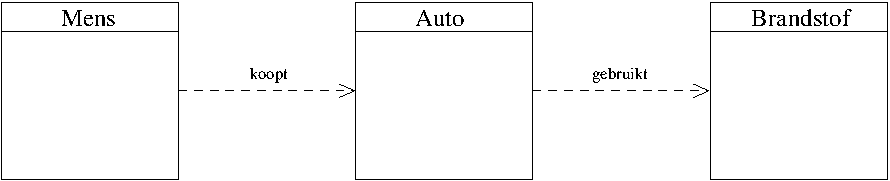
\includegraphics[width=11cm]{asso}  
\end{center}
\end{frame}


\begin{frame}\frametitle{Aggregatie}
De ene klasse kan als attribuut een andere klasse hebben.
\vspace{0.5cm}
   \begin{center}
  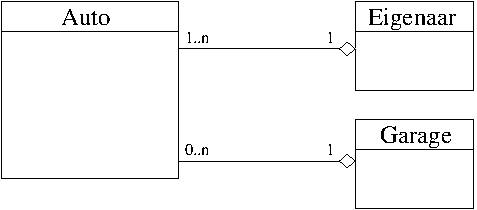
\includegraphics[height=3cm]{aggr}  
\end{center}
\begin{itemize}
\item Een eigenaar heeft 1 of meerdere auto' s.
\item Een auto heeft \'e\'en eigenaar.
\end{itemize}
\end{frame}


\begin{frame}
\frametitle{Compositie}
\begin{center}
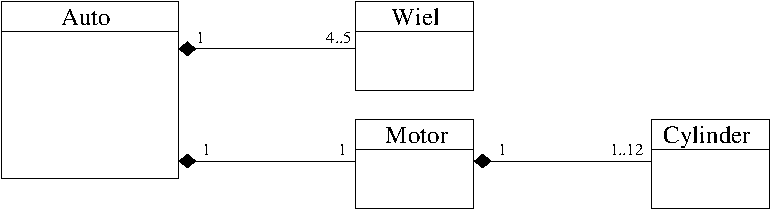
\includegraphics[width=10cm]{compo}
\end{center}
\href{http://en.wikipedia.org/wiki/Bond_Minicar}{Bond minicar 1949}\\
\href{http://en.wikipedia.org/wiki/Pullman_automobile}{Pullman 1905}
\end{frame}

\begin{frame}\frametitle{Compositie vs. aggregatie}
Compositie:
  \begin{itemize}
  \item dichte diamanten
  \item het ene object kan niet bestaan zonder het andere.
  \item het ene obect is een onderdeel van het andere
  \item voorbeeld: huis$\leftrightarrow$muur\pause
  \end{itemize}
Aggregatie:
\begin{itemize}
  \item open diamanten
  \item het ene object kan bestaan zonder het andere
  \item voorbeeld: vereniging$\leftrightarrow$leden
\end{itemize}
\end{frame}

\begin{frame}\frametitle{Subtyping}
Class deriving van een concrete parent class.
\begin{center}
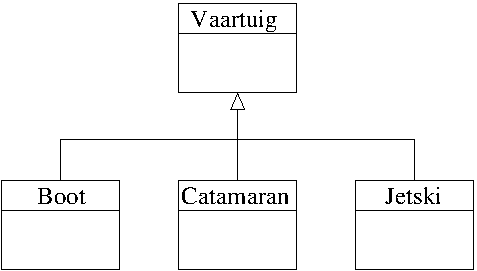
\includegraphics[width=8cm]{subt}
\end{center}  
\end{frame}

\begin{frame}
\frametitle{Subtyping}
Class deriving van een abstracte parent class.
\begin{center}
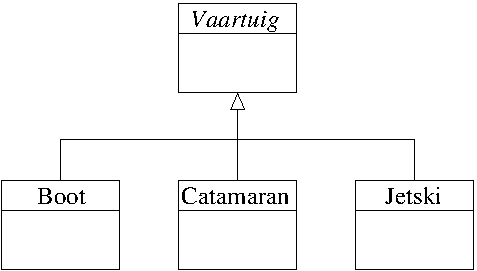
\includegraphics[width=8cm]{subt2}
\end{center}  

\end{frame}


\end{document}